\section{Implementierung}

\subsection {Inbetriebnahme Greifarm}
Der OMX wird als Bausatz geliefert.Für die Inbetriebnahme ist daher der Zusammenbau und die Installation der entsprechenden Software  nötig. 
\subsubsection{Zusammenbau}
-Bausatz ca 40 Teile (ohne Schrauben)\\
-Rausbrechen Plastik bei Vorbereitung Servos\\
-Servos einzeln anschließen und per Dynamixel Wizard ID setzen\\
Der Bausatz des OMX besteht aus ca. 60 Teilen (ohne Schrauben, s. Abbildung \ref{fig:omxparts}).Einige der mit den Servomotoren mitgelieferten Teile werden dabei nicht benötigt, da der Bausatz des OMX diese auch enthält oder ersetzt (z.B. längere Kabel). Von allen Schrauben wurde außerdem Ersatz mitgeliefert.\\
Der Zusammenbau erfolgte nach der auf der Webseite verfügbaren Bauanleitung VERWEIS ANLEITUNG. Zu beachten ist, dass hier vorrausgesetzt wird, dass den Servos bereits die IDs 11 (Basis des Greifarms) bis 15 (Greifer) zugewiesen wurden. Dies kann über die Software DYNAMIXEL Wizard{\footnote{VERWEIS ODER LINK}} gemacht werden: die Servos einzeln über das U2D2 (s. Abschnitt {\ref{u2d2}}) an den PC anschließen, die ID setzen und den Servo entsprechend markieren oder die ID merken. Weiterhin müssen bei den Abdeckungen der Servos 12 und 14 die vorgestanzten Abdeckungen herausgebrochen werden. Dies ist in der Anleitung leicht zu übersehen. Weiterhin wird angenommen, dass das Horn der Servos bereits angebracht ist. Hierbei ist darauf zu achten, dass die Einkerbung an Horn und Servo übereinstimmen.
\begin{figure}[ht!]
\centering
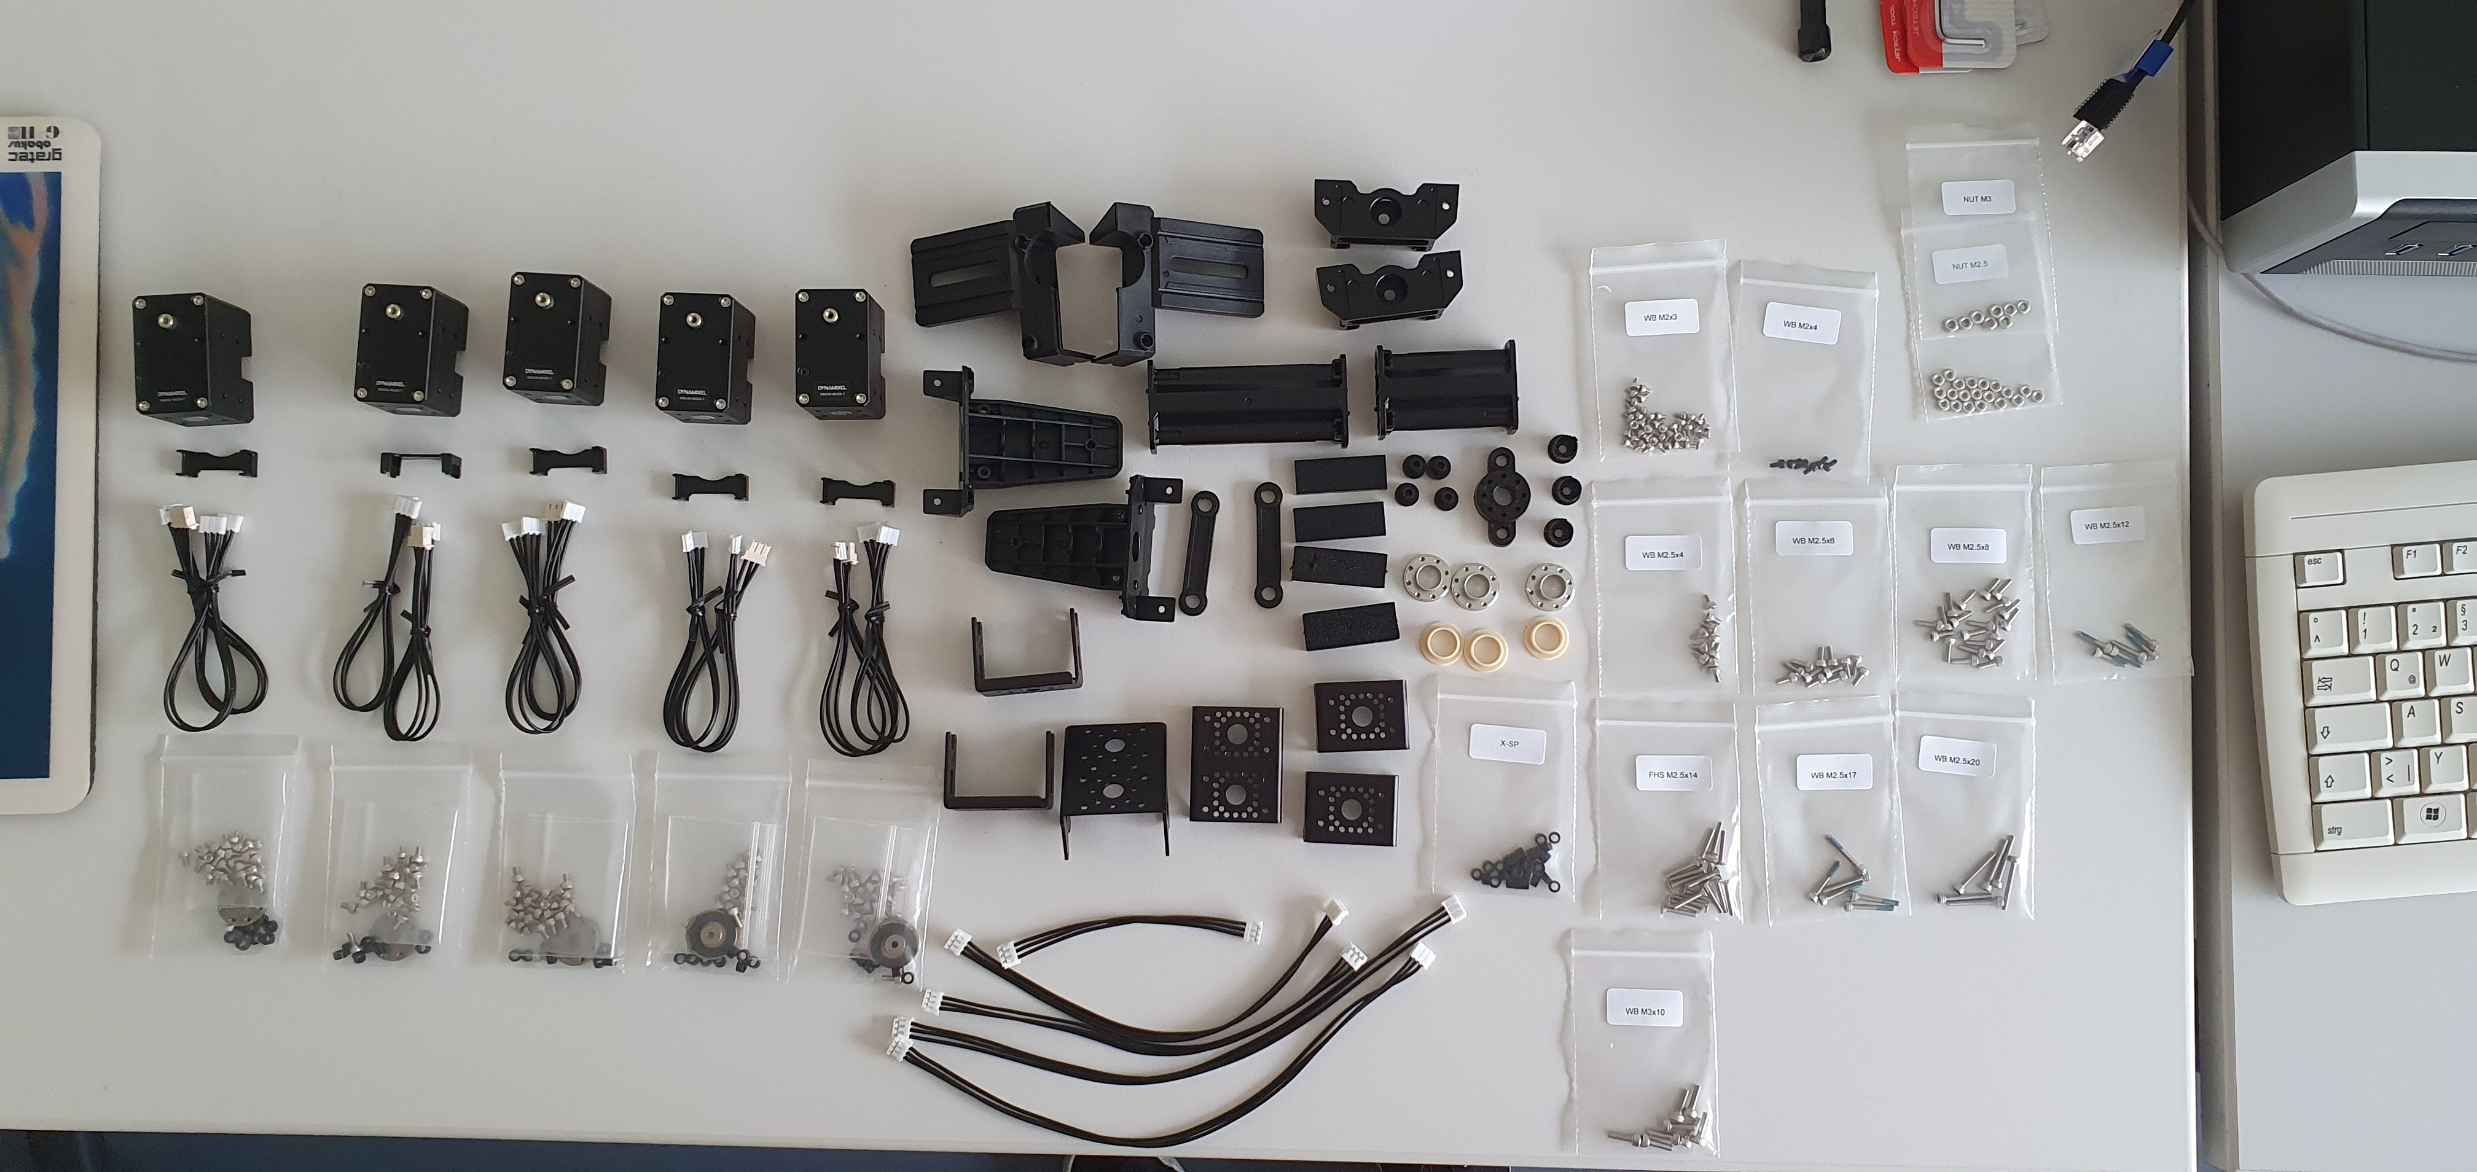
\includegraphics[width=\textwidth]{parts.jpg}
\caption{Bausatz für den OpenMANIPULATOR-X}
\label{fig:omxparts}
\end{figure}
\subsubsection{Virtuelle Maschine}
-Ubuntu 20.04\\
-- Auflösung Einstellung "keine"\\
-Installation ROS2 Foxy\\
-Installation OMX\\
Zur Nutzung des Greifarms wurde eine \ac{VM} mit VirtualBox {\footnote{https://www.virtualbox.org}} von Oracle aufgesetzt. Als Betriebssystem der \ac{VM} wurde das für ROS2 Foxy empfohlene \citep{foxyreq} Ubuntu 20.04 {\footnote{\url{https://releases.ubuntu.com/20.04/}}} gewählt. Danach wurde entsprechend der Anleitung für den OpenMANIPULATOR-X \citep{foxyinstall} zuerst ROS 2 Foxy über das Installations-Script von ROBOTIS und im Anschluss die für den Greifarm benötigten Packages installiert.
\subsection{Steuerung OMX}
Die Steuerung des OMX erfolgt über die vom \emph{open\_manipulator\_x\_controller}\\ \verb|open_manipulator_x_controller| zur Verfügung gestellten Topics und Services.
\subsubsection{Anschluss über U2D2}{\label{u2d2}}
Der OMX wird über das U2D2 und das U2D2 Power Hub Board (s. Abbildung \ref{fig:u2d2}) per USB an den PC angeschlossen.\\
Das U2D2 konvertiert die Signale der DYNAMIXEL und ermöglicht die Kontrolle über den PC. Zur Nutzung des U2D2 in der \ac{VM} muss das Gerät FTDI XXXXXXXXX über das Geräte-Menü der \ac{VM} an diese gebunden werden (s. Abbildung \ref{fig:ftdivm}).
\begin{figure}[ht!]
\centering

\includegraphics[width=\textwidth]{u2d2.png}
\caption{U2D2 Power Hub Board mit montiertem U2D2 (LINKS/RECHTS im Bild)}
\label{fig:u2d2}
\end{figure}
\begin{figure}[ht!]
\centering

\includegraphics[width=\textwidth]{ftdivm.png}
\caption{Geräte-Menü der \ac{VM} mit gebundenem U2D2}
\label{fig:ftdivm}
\end{figure}
\subsubsection{OMX-Controller}
Der OMX-Controller ist ein Package, welches automatisch beim Installieren der für den OMX benötigten Software installiert wird. Er kann über die entsprechende Launch-Datei mit dem Befehl
\begin{verbatim}
ros2 launch open_manipulator_x_controller 
     open_manipulator_x_controller.launch.py
\end{verbatim}
gestartet werden.
\subsubsection{Topics}
\subsubsection{Kinematik}
\subsubsection{Teleop} \label{teleop}
Mit einem laufenden OMX-Controller kann der OMX auch ohne extra Programmierung direkt ferngesteuert werden. Mögliche Geräte zur Steuerung sind die Tastatur sowie Playstation- und XBOX-Controller. Für \ac{ROS2} Foxy wird aktuell allerdings nur die Steuerung über die Tastatur unterstützt.\\
Der OMX kann dabei sowohl im Task Space als auch im Joint Space kontrolliert werden (s. Abbildung \ref{fig:teleopkeyboard}). Zusätzlich gibt es 2 vordefinierte Posen (Init und Home) in die der OMX bewegt werden kann (s. Abbildung \ref{fig:teleopposes}).
\begin{figure}[ht!]
\centering
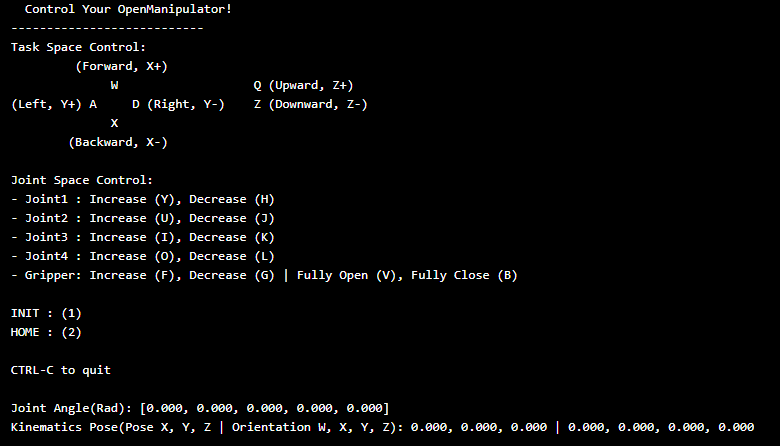
\includegraphics[width=\textwidth]{teleopkeyboard.png}
\caption{Fernsteuerung des OMX über die Tastatur}
\label{fig:teleopkeyboard}
\end{figure}
\begin{figure}[htb]
    \centering
    \begin{minipage}[t]{0.45\linewidth}
        \centering
        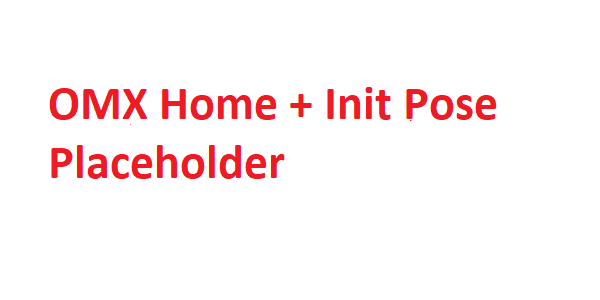
\includegraphics[width=\linewidth]{omxposes}
    \end{minipage}% <- sonst wird hier ein Leerzeichen eingefügt
    \hfill
    \begin{minipage}[t]{0.45\linewidth}
        \centering
        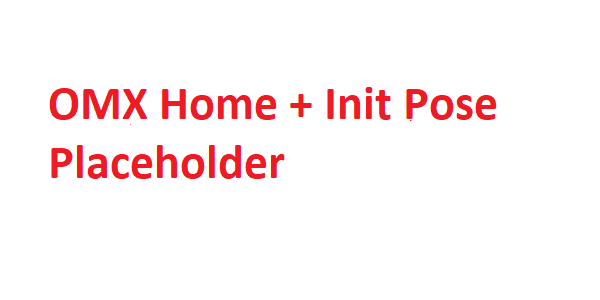
\includegraphics[width=\linewidth]{omxposes}
    \end{minipage}
    \caption{Home (l.) und Init (r.) Pose der Tastatur Teleop}
    \label{fig:teleopposes}
\end{figure}
\subsection{PlanSys2}
\cite{plansys}\\
Für die Implementierung der in \ref{konzept:nodes} genannten Funktionalitäten wird das Framework \ac{PlanSys2} genutzt. Es übernimmt dabei alle Funktionalitäten: die Verwaltung der Daten zur Domäne und dem aktuellen Problem erfolget über die domain-expert und problem-expert Nodes. Die planer Node ist für die komplette Planung zuständig und die Executioner Node für die Ausführung des Plans.\\
Es müssen hier lediglich die Domäne erstellt sowie die tatsächliche Funktionalität der einzelnen Aktionen implementiert werden. Das Wort Action im Namen der Nodes und den folgenden Kapiteln bezieht sich hier auf die Aktionen der Domäne, nicht auf \ac{ROS2} Actions.
\subsubsection{PDDL-Domain}
-Durative Actions\\
-Gripper + Blockworld\\
- keine existential/negative Preconditions\\
Beim erstellen der Domäne ist zu beachten, das \ac{popf} nicht alle Funktionen unterstützt, die mit PDDL beschrieben werden können. Dies beinhaltet unter anderem existentielle sowie negative Vorbedingungen. Die vollständige Liste ist auf \ref{popfpddlsupport} zu finden.\\
Für den Blockworld Teil der Domäne gibt es zunächst den Typ \verb|box| und Prädikate, die das Stapeln von Blöcken darstellen. Dies umfasst das Verhältnis von Blöcken aufeinander (\verb|(box_on ?b_above ?b_below - box)|) sowie ob ein Block der oberste eines Stapels und damit frei zum bewegen ist (\verb|(clear ?b - box)|). Als Aktionen werden das Nehmen sowie Ablegen eines Blocks benötigt. Da in den Bedingungen und Effekten einer Aktion nur mit Parametern gearbeitet werden kann, welche auch Parameter der Aktion selbst sind, wird hier weiter aufgeteilt in Nehmen/Ablegen eines Blocks von/auf einen anderen Block sowie von/auf einen leeren Stapel. Für das Bewegen von Blöcken ergeben sich die 4 Aktionen \verb|GRAB, PLACE, STACK, UNSTACK|.\\
Während für das reine Stapeln der Blöcke die exakte Position dieser nicht wichtig ist, wird diese jedoch für den Greifer benötigt, welcher vor diesen Aktionen an die richtige Stelle bewegt werden muss. Hier werden die weiteren Typen \verb|location| und \verb|stack| sowie die Prädikate \verb|(box_at ?b - box ?l - location)|,\\ \verb|(gripper_at ?g - gripper ?l - location)|,\\ \verb|(location_above ?l_above ?l_below - location)| und\\ \verb|(is_base_loc ?l - location ?s - stack)| eingeführt.\\ \\
Das Prädikat \verb|clear| ist notwendig, da \ac{POPF} weder existentielle noch negative Vorbedingungen unterstützt. Es wird genutzt um zu überprüfen, ob ein Block der oberste eines Stapels ist, was es ermöglicht diesen zu nehmen oder einen anderen auf diesem abzulegen.Durch existentielle und negative Vorbedingungen könnte dies für die Aktion den Block B zu greifen, durch eine Bedingung der Form ''es existiert kein Block C für den gilt:( box\_on C B)'' ersetzt werden. \\ \\
Da alle Aktionen eine Dauer haben und \ac{PlanSys2} auch nur diese unterstützt, werden alle Aktionen als \verb|durative-action| modelliert. Es wird jeder Aktion eine Dauer zugeordnet (\verb|:duration (= ?duration 0.25)|) welche auch für Metriken genutzt werden kann. Zusätzlich bekommen Bedingungen und Effekte einen temporalen Zusatz: \verb|at start| und \verb|at end| können sowohl für Bedingungen als auch Effekte benutzt werden um festzulegen zu welchem Zeitpunkt der Aktion diese Bedingung zutreffen oder der Effekt eintritt. Für Bedingungen gibt es außerdem \verb|over all| damit eine Bedingung über die komplette Dauer der Aktiion zutreffen muss damit sie gültig ist.\\
Im aktuellen Szenario wird \verb|over all| dafür genutzt, allen Block-Aktionen die Bedingung zu geben, dass sich der Greifer über die komplette Zeit an der gleichen Stelle wie der entsprechende Block befinden muss.\\
Nur in der \verb|MOVE-GRIPPER| Aktion wird \verb|at start| für einen Effekt genutzt: \verb|(at start(not (gripper_at ?g ?l_from)))|. Sobald die Aktion beginnt befindet sich der Greifer nicht mehr an der Ausgangsposition und erst am Ende der Aktion wird die neue Position als Fakt gesetzt (\verb| (at end(gripper_at ?g ?l_to))|), Würden beide Effekte erst am Ende der Aktion eintreten, würde der Planer mehrere \verb|MOVE-GRIPPER| Aktionen parallel ausführen (s. Abbildung \ref{fig:tempgrippereffect}). Dies ist zum einen physisch nicht möglich, hinterlässt die Welt aber auch in einem ungültigen Zustand, da der Greifer sich dann an mehreren Positionen gleichzeitig befinden würde.
\subsubsection{Action Nodes}
Obwohl in der Domäne mehr als 2 Aktionen beschrieben sind, beschränken sich die ausgeführten Aktionen auf ein Bewegen des OMX sowie die Kontrolle des Greifers. Für diese wird jeweils eine Node erstellt. Damit diese Nodes von \ac{PlanSys2} genutzt werden können müssen sie von der Basisklasse \verb|plansys2::ActionExecutorClient| erben. Da diese von \ac{PlanSys2} nur in C++ zur Verfügung gestellt wird, müssen auch die Aktionen in C++ implementiert werden.\\
In jeder Aktion muss die Methode \verb|void do_work()| implementiert werden. Diese wird mit einem bestimmten Zeitintervall aufgerufen während die Aktion aktiv ist. Das Intervall wird im Konstruktor gesetzt (s. Zeile \ref{code:line:nodeintervall} in \ref{code:gripperactionnode}). Das Mapping einer Node zu einer Aktion erfolgt durch das Setzen des Parameters \verb|action_name| nach dem Erstellen der Node (s. Zeile \ref{code:line:actionname} in \ref{code:gripperactionnode}).
\subsubsection{Move Gripper Aktion}
\subsubsection{Control Gripper Aktion}
Die Logik Node zur Steuerung des Greifers wird in der Klasse \verb|ControlGripperAction| (s. \ref{code:gripperactionnode}) implementiert. Da es vom OMX kein Feedback gibt, ob oder wann etwas gegriffen wurde, wird die Aktion mit einer fixen Wartezeit implementiert: wenn die Aktion gestartet wird, wird ein Request zur Steuerung des Greifers erzeugt (s. Zeile \ref{code:line:gripperrequest} in \ref{code:gripperactionnode}) und gesendet und nach einer bestimmten Zeit die Aktion beendet. Um unnötige Aufrufe der Methode während des Wartens zu verhindern wird die Wartezeit über das Zeitintervall zur Ausführung der Node gesetzt. Die Aktion wird hierdurch immer beim 2. Aufruf der Methode \verb|do_work| beendet.\\
Zum Senden des Requests wird ein \ac{ROS2} Client für den Service \verb|goal_tool_control| mit dem Typ \verb|open_manipulator_msgs::srv::SetJointPosition| erstellt. 
Um sowohl die Aktionen zum Öffnen sowie Schließen des Greifers mit einer Node implementieren zu können wird ein Parameter eingeführt, welcher über die Launch-Datei gesetzt wird und die Bewegung des Greifers bestimmt.
\subsection{Praktisches Bsp}

%\newpage